\subsection{How much of the shortlist survives a change of sample or seed?}
The validation sample contains 567 ordered metal pairs. Each pair contributes seven associated families, and we use the pair as the resampling unit. To assess sensitivity to the mix of pairs, we draw 567 pairs with replacement, retaining the whole family group and its multiplicity. On each resample we rank the records using the already fitted seed-26 predictors and count $V<1$ hits among the first 50. Figure~\ref{fig:stability} uses the same draw for both methods. This paired design preserves the dependence of their predictions on the same materials.

\begin{figure}[htbp]
\centering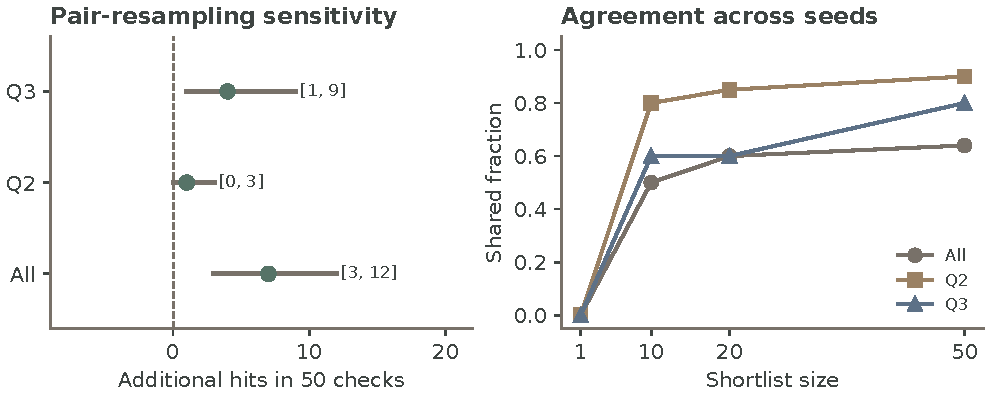
\includegraphics[width=\linewidth]{figures/validation_stability.pdf}
\caption{Left, observed mixture-minus-direct hit counts at budget 50 (dots) and the 2.5th to 97.5th percentiles over 2,000 resampled pair sets (segments). Right, the fraction of each mixture shortlist shared by training seeds 26 and 42 on the original validation set.}\label{fig:stability}
\end{figure}

Across all families the observed improvement is seven hits, with a resampling range of three to twelve. For Q2 the improvement is one and the interval reaches zero. Only four near-targets are present in that validation pool, leaving little room for a large observed gain. For Q3 the gain is four with a range of one to nine. The intervals describe sensitivity conditional on the trained models and the empirical pair distribution. Resampled duplicates count toward both hit totals and the 50-record budget. These are diagnostics of the metric, rather than prospective yields for 50 distinct new experiments.

We separately intersect the predicted shortlists from seeds 26 and 42. At $k=50$, 45 of 50 Q2 candidates and 40 of 50 Q3 candidates are shared. At $k=1$ the two seeds select different IDs in both pools. We therefore report the first choice on the frozen score table together with its validation regret. Seed agreement at a larger budget supports a follow-up shortlist but supplies little assurance about which single material a laboratory should measure first.
